% =====================================================================
%  答辩幻灯 · 演讲者备注版（Beamer notes / 演讲者视图）
%  每页输出 = 幻灯（左）+ 备注（右），供 pdfpc / 双屏演讲者模式或对照排练
%  排版优化版：阶段导览 + 每页结论 + 统一字体层级 + 汇报逻辑重排
% =====================================================================
\documentclass[aspectratio=169,fontset=none,11pt]{ctexbeamer}

\setCJKmainfont{Noto Sans CJK SC}
\setCJKsansfont{Noto Sans CJK SC}
\setCJKmonofont{Noto Sans Mono CJK SC}

\usepackage{tikz}
\usetikzlibrary{positioning,arrows.meta,calc,fit}
\usepackage{listings}
\usepackage{pifont}
\usepackage{booktabs}
\usepackage{qrcode}

\graphicspath{{../docs/screenshots/}{../docs/field/}}

% ---------------- 配色 ----------------
\definecolor{abbred}{RGB}{217,74,31}
\definecolor{abbdark}{RGB}{28,28,28}
\definecolor{abbgray}{RGB}{110,110,110}
\definecolor{abblight}{RGB}{246,242,240}
\definecolor{boxblue}{RGB}{226,236,246}
\definecolor{consolebg}{RGB}{20,24,28}
\definecolor{consolefg}{RGB}{224,228,232}
\definecolor{okgreen}{RGB}{34,140,64}

% ---------------- 主题与字体层级 ----------------
\usetheme{default}
\setbeamertemplate{navigation symbols}{}
\setbeamercolor{structure}{fg=abbred}
\setbeamercolor{frametitle}{fg=abbdark}
\setbeamercolor{title}{fg=abbdark}
\setbeamercolor{itemize item}{fg=abbred}
\setbeamercolor{itemize subitem}{fg=abbgray}
\setbeamerfont{frametitle}{series=\bfseries,size=\LARGE}
\setbeamerfont{itemize/enumerate body}{size=\normalsize}
\setbeamerfont{itemize/enumerate subbody}{size=\small}
\setbeamertemplate{itemize item}{\small\ding{228}}
\setbeamertemplate{itemize subitem}{\textemdash}
\linespread{1.06}

% 阶段导航条（顶部进度条，当前阶段自动点亮）
\newcommand{\curphase}{0}
\newcommand{\navseg}[2]{\ifnum\curphase=#1\relax{\color{abbred}\bfseries #2}\else{\color{abbgray}#2}\fi}
\setbeamertemplate{headline}{%
  \ifnum\curphase>0\relax
    \vskip5pt\hbox to\paperwidth{\hfill\scriptsize\sffamily
      \navseg{1}{\ding{172}\,背景与方案}\hskip5pt{\color{abbgray!45}\textbar}\hskip5pt
      \navseg{2}{\ding{173}\,系统与关键技术}\hskip5pt{\color{abbgray!45}\textbar}\hskip5pt
      \navseg{3}{\ding{174}\,工程与现场验证}\hskip5pt{\color{abbgray!45}\textbar}\hskip5pt
      \navseg{4}{\ding{175}\,创新与总结}\hskip12pt}\vskip-3pt
  \fi}
\setbeamertemplate{frametitle}{%
  \vspace{2pt}{\usebeamerfont{frametitle}\insertframetitle}\par\vspace{2pt}%
  {\color{abbred}\rule{0.34\paperwidth}{1.4pt}}\par\vspace{-3pt}}
\setbeamertemplate{footline}{%
  \hbox{\begin{beamercolorbox}[wd=\paperwidth,ht=2.4ex,dp=1.2ex,leftskip=10pt,rightskip=10pt]{}%
  {\color{abbgray}\scriptsize 人工智能创新赛 · abb-offline-coder\hfill 队伍：人工智能创新001\hfill\insertframenumber/\inserttotalframenumber}%
  \end{beamercolorbox}}}

% 结论条
\newcommand{\takeaway}[1]{%
  \vfill
  \begin{tikzpicture}
  \node[fill=abbred!12,rounded corners=3pt,inner sep=6pt,
        text width=\dimexpr\textwidth-14pt\relax]
       {\small\textbf{\color{abbred}结论\,}\ #1};
  \end{tikzpicture}\vspace{-1pt}}

% ====== 演讲者备注：每页输出 幻灯(左) + 备注(右) ======
\usepackage{pgfpages}
\setbeameroption{show notes on second screen=right}
\setbeamerfont{note page}{size=\small}
\setbeamercolor{note page}{bg=white,fg=abbdark}
\setbeamertemplate{note page}{%
  \vskip8pt\hskip10pt{\color{abbred}\bfseries\large 演讲者备注}%
  \hfill{\color{abbgray}\small 第 \insertframenumber\ /\,\inserttotalframenumber\ 页}\hskip10pt\par
  \vskip3pt\hskip10pt{\color{abbred}\rule{0.42\paperwidth}{1.2pt}}\par\vskip6pt
  \hskip10pt\begin{minipage}{0.86\paperwidth}\setlength{\parskip}{4pt}\small\insertnote\end{minipage}}

% ---------------- 代码样式 ----------------
\lstdefinestyle{rapidmini}{
  backgroundcolor=\color{abblight},basicstyle=\ttfamily\scriptsize,
  keywordstyle=\color{abbred}\bfseries,commentstyle=\color{abbgray}\itshape,
  morekeywords={MODULE,ENDMODULE,PROC,ENDPROC,PERS,CONST,MoveL,PaintL,SetDO,ConfL,SingArea},
  comment=[l]{!},breaklines=true,columns=fullflexible,frame=none,xleftmargin=4pt}
\lstdefinestyle{con}{backgroundcolor=\color{consolebg},
  basicstyle=\ttfamily\scriptsize\color{consolefg},breaklines=true,
  columns=fullflexible,frame=none,xleftmargin=4pt}

\newcommand{\redb}[1]{{\color{abbred}\bfseries #1}}

\tikzset{
  blk/.style={draw=abbdark,line width=0.6pt,rounded corners=2pt,fill=white,
    align=center,font=\scriptsize,minimum height=0.8cm,inner sep=2pt},
  hot/.style={draw=abbred,line width=0.9pt,fill=abblight,rounded corners=2pt,
    align=center,font=\scriptsize\bfseries,minimum height=0.8cm,inner sep=2pt},
  fl/.style={-{Latex[length=1.6mm]},line width=0.7pt,abbred},
}

\begin{document}

% ============ 封面 ============
{\setbeamertemplate{footline}{}
\begin{frame}[plain]
  \begin{tikzpicture}[remember picture,overlay]
    \fill[abbred] ([yshift=-1.0cm]current page.north west) rectangle (current page.north east);
    \fill[abblight] (current page.south west) rectangle ([yshift=1.3cm]current page.south east);
  \end{tikzpicture}
  \vfill
  \begin{center}
  {\color{abbgray}\sffamily 人工智能创新赛 · 项目答辩}\\[10pt]
  {\fontsize{36}{40}\selectfont\bfseries abb-offline-coder}\\[4pt]
  {\color{abbred}\rule{4cm}{2pt}}\\[8pt]
  {\Large 面向 ABB 喷涂机器人的离线 AI 编程助手}\\[6pt]
  {\color{abbgray} “把中文一句话变成 ABB RAPID 喷涂程序”}\\[16pt]
  {\large 队伍：\textbf{人工智能创新001}}\\[2pt]
  {\color{abbgray}\small 完全离线 · 本地 LLM + 官方手册 RAG · 工业 PC 断网可用}
  \end{center}
  \vfill
  \note{\textbf{开场（约 30 秒）}：向评委问好；报清队名「人工智能创新001」与项目名 abb-offline-coder。\\
  一句话定位：把\textbf{中文一句话}变成\textbf{可直接上机}的 ABB RAPID 喷涂程序，而且\textbf{全程不联网}。\\
  \textit{提示：开场放稳、语速略慢；目光扫视全体评委后再翻页。}}
\end{frame}}

% ============ 汇报提纲 ============
\begin{frame}{汇报提纲}
\vspace{2pt}
\begin{columns}[T]
\begin{column}{0.5\textwidth}
{\large\textbf{\color{abbred}\ding{172} 背景与方案}}\\[2pt]
\hspace{1em}行业痛点 \;$\to$\; 解决方案与定位\\[14pt]
{\large\textbf{\color{abbred}\ding{173} 系统与关键技术}}\\[2pt]
\hspace{1em}四层架构 + 六级流水线\\
\hspace{1em}领域 RAG · 生成—校验闭环 · 双控制器
\end{column}
\begin{column}{0.5\textwidth}
{\large\textbf{\color{abbred}\ding{174} 工程与现场验证}}\\[2pt]
\hspace{1em}实测佐证 · 应用案例 · 真实现场\\[14pt]
{\large\textbf{\color{abbred}\ding{175} 创新与总结}}\\[2pt]
\hspace{1em}创新点总览 · 价值与展望
\end{column}
\end{columns}
\takeaway{一条主线——\textbf{现场无网的真痛点 $\to$ 完全离线方案 $\to$ 技术实现 $\to$ 实测与现场验证 $\to$ 价值}。}
\note{\textbf{导览（约 20 秒）}：先给评委一条主线，让后面有预期——\textbf{痛点 $\to$ 方案 $\to$ 技术 $\to$ 验证 $\to$ 价值}。\\
\textit{提示：一句话带过，不逐条念；点出“四个部分”即可翻页。}}
\end{frame}

% ====================================================================
\renewcommand{\curphase}{1}
% ============ 1. 痛点 ============
\begin{frame}{行业痛点：喷涂编程的“三高一隔离”}
\begin{columns}[T]
\begin{column}{0.56\textwidth}
\begin{itemize}
  \item \redb{门槛高}：RAPID 专有语言，喷涂还叠加笔刷工艺、喷枪时序、TCP 标定、IO 配置
  \item \redb{试错贵}：信号没注册上机即报 \texttt{40212}；TCP 没标定可能撞机
  \item \redb{依赖人}：培养独立编程工程师以\textbf{月}计
  \item \redb{现场隔离}：喷涂车间多为\textbf{物理隔离、完全无网}
\end{itemize}
\end{column}
\begin{column}{0.44\textwidth}
\begin{tikzpicture}
\node[draw=abbred,line width=1pt,rounded corners=4pt,fill=abblight,inner sep=8pt,
      text width=\dimexpr\linewidth-18pt\relax,font=\small]{%
\textbf{云端 AI 编程工具}（Copilot / ChatGPT / Cursor）\textbf{在喷涂现场根本无法落地}，
现场数据也\textbf{不允许外传}。};
\end{tikzpicture}
\end{column}
\end{columns}
\takeaway{云端工具用不了、数据不能外传 $\Rightarrow$ 需要一个\textbf{完全离线、又懂喷涂}的中文 AI 编程助手。}
\note{\textbf{痛点（约 50 秒）—— 三高一隔离}：\\
\textbf{\ding{172}门槛高}：RAPID 专有语言 + 喷涂工艺/时序/标定/IO；\textbf{\ding{173}试错贵}：信号没注册上机报 \texttt{40212}；
\textbf{\ding{174}依赖人}：培养工程师以月计；\textbf{\ding{175}现场隔离}：车间物理无网。\\
落点：云端工具用不了、数据不能外传 $\Rightarrow$ 必须\textbf{完全离线、又懂喷涂}。\\
\textit{提示：“三高一隔离”重读；念到 40212 停半拍，强调是“现场真问题”。}}
\end{frame}

% ============ 2. 方案与定位 ============
\begin{frame}{解决方案与定位}
\begin{center}
\itshape\large “把中文一句话变成 ABB RAPID 喷涂程序——\\本地小模型 + 官方手册 RAG，工业 PC 断网可用。”
\end{center}
\vspace{6pt}
\begin{columns}[T]
\begin{column}{0.5\textwidth}
\textbf{\color{abbred}做什么}\\[3pt]
用户用\textbf{中文}描述喷涂需求，系统直接产出符合 ABB 规范、可导入 RobotStudio 的 \texttt{.mod} 程序。
\end{column}
\begin{column}{0.5\textwidth}
\textbf{\color{abbred}怎么做到离线}
\begin{itemize}
  \item 本地量化 LLM（Qwen2.5-Coder，CPU 可跑）
  \item 官方手册 RAG（向量 + BM25 混合检索）
  \item 数据\textbf{全程不出厂}
\end{itemize}
\end{column}
\end{columns}
\takeaway{中文一句话 $\to$ 可上机 \texttt{.mod}；\textbf{本地模型 + 手册 RAG + 数据不出厂}，云端工具做不到。}
\note{\textbf{方案（约 35 秒）—— 电梯演讲}：中文一句话 $\to$ RAPID 喷涂程序。\\
能离线靠三点：\textbf{\ding{172}本地量化模型 CPU 可跑}；\textbf{\ding{173}官方手册 RAG}；\textbf{\ding{174}数据不出厂}。\\
\textit{提示：节奏明快、自信；三点可掰手指强调。}}
\end{frame}

% ====================================================================
\renewcommand{\curphase}{2}
% ============ 3. 系统设计 ============
\begin{frame}{系统设计：四层架构 + 六级流水线}
\begin{columns}[T]
\begin{column}{0.46\textwidth}
\centering\footnotesize\textbf{\color{abbred}四层架构}\\[3pt]
\begin{tikzpicture}
\node[blk,fill=abblight,text width=4.3cm] (c){CLI 层 · gen/chat/kb/...};
\node[blk,fill=boxblue,text width=4.3cm,below=3pt of c](o){编排层 Agent · 流水线};
\node[hot,minimum width=1.3cm,below=11pt of o.south,xshift=-1.6cm](r){rag/};
\node[hot,minimum width=1.3cm,below=11pt of o.south](l){llm/};
\node[hot,minimum width=1.3cm,below=11pt of o.south,xshift=1.6cm](p){rapid/};
\node[blk,fill=abblight,text width=4.3cm,below=11pt of l](k){knowledge/ → ChromaDB};
\draw[fl](c)--(o);\draw[fl](o.south)--(r.north);\draw[fl](o)--(l);\draw[fl](o.south)--(p.north);\draw[fl](r)--(k);
\end{tikzpicture}
\end{column}
\begin{column}{0.54\textwidth}
\centering\footnotesize\textbf{\color{abbred}六级生成流水线}\\[3pt]
\begin{tikzpicture}[node distance=4pt]
\node[hot,text width=2.0cm](q){中文需求};
\node[blk,text width=2.0cm,right=4pt of q](a){\ding{172} 查询改写};
\node[blk,text width=2.0cm,below=4pt of a](b){\ding{173} 混合检索};
\node[blk,text width=2.0cm,left=4pt of b](cc){\ding{174} 上下文装配};
\node[blk,text width=2.0cm,below=4pt of cc](d){\ding{175} 本地 LLM};
\node[blk,text width=2.0cm,right=4pt of d](e){\ding{176} 校验后处理};
\node[hot,text width=2.0cm,below=4pt of e](f){\ding{177} .mod 输出};
\draw[fl](q)--(a);\draw[fl](a)--(b);\draw[fl](b)--(cc);\draw[fl](cc)--(d);\draw[fl](d)--(e);\draw[fl](e)--(f);
\end{tikzpicture}
\end{column}
\end{columns}
\takeaway{纯函数流水线、数据不可变，副作用集中在 Ollama/ChromaDB 边界 $\to$ \textbf{易测、可演进、能离线}。}
\note{\textbf{系统设计（约 50 秒）}：左边\textbf{四层架构}（CLI / 编排 Agent / 三能力模块 rag·llm·rapid / 知识库）；
右边\textbf{六级流水线}：需求 $\to$ 改写 $\to$ 检索 $\to$ 装配 $\to$ 本地 LLM $\to$ 校验后处理 $\to$ .mod。\\
强调：\textbf{纯函数、数据不可变、副作用集中在 Ollama/ChromaDB 边界} $\Rightarrow$ 好测、可演进、能离线。\\
\textit{提示：左右两张图各指一下；“边界”二字重读，为后面高覆盖率埋伏笔。}}
\end{frame}

% ============ 4. 关键技术 ============
\begin{frame}[fragile]{关键技术：领域 RAG + 生成—校验闭环}
\begin{columns}[T]
\begin{column}{0.5\textwidth}
\textbf{\color{abbred}\ding{172} 领域专精 RAG（抑制幻觉）}
\begin{itemize}\small
  \item 10 本官方手册 → \textbf{7497} 片段向量库
  \item 向量 + BM25 混合：$\alpha\hat s_{vec}+(1{-}\alpha)\hat s_{bm25}$
  \item 让小模型也能正确引用 \texttt{MToolTCPCalib}、\texttt{TriggIO}
\end{itemize}
\end{column}
\begin{column}{0.5\textwidth}
\textbf{\color{abbred}\ding{173} 生成—校验闭环（安全护栏）}
\begin{itemize}\small
  \item 11 类静态校验 + 可追溯错误码
  \item 把现场高代价错误\textbf{左移到生成时拦截}
\end{itemize}
\vspace{3pt}
\begin{lstlisting}[style=con]
[ERROR][PNT001] 缺 brushdata 形参
[ERROR][IO001]  信号不在 EIO.cfg 白名单
\end{lstlisting}
\end{column}
\end{columns}
\takeaway{RAG 让小模型\textbf{查得到、不乱编}；校验闭环把现场 \texttt{40212} 类错误\textbf{提前到生成时}拦下。}
\note{\textbf{关键技术（约 55 秒，含金量最高、可放慢）}：\\
\textbf{\ding{172}领域 RAG}：10 本手册 $\to$ 7497 片段，\textbf{向量 + BM25 混合}；让 7B 小模型也能正确引用
\texttt{MToolTCPCalib}、\texttt{TriggIO} 这种它本不知道的指令，\textbf{抑制幻觉}。\\
\textbf{\ding{173}生成—校验闭环}：11 类校验 + 错误码；漏 brushdata 报 \textbf{PNT001}，未注册信号报 \textbf{IO001}
= 把现场才暴露的 \texttt{40212} \textbf{左移到生成时}。\\
\textit{提示：念错误码时指右下角黑底实录。}}
\end{frame}

% ============ 5. 双控制器 + Pack&Go ============
\begin{frame}{双控制器自适应 + Pack\&Go 一键交付}
\begin{columns}[T]
\begin{column}{0.56\textwidth}
\textbf{\color{abbred}IRC5 / IRC5P 一键切换}\\[3pt]
同一句话，按控制器产出不同工艺风格：
\begin{itemize}\small
  \item \textbf{IRC5}：\texttt{MoveL + SetDO} 手动开关枪
  \item \textbf{IRC5P}：\texttt{PaintL/PaintC + brushdata} 原生工艺
\end{itemize}
\texttt{controller} 是贯穿\,提示词/生成/校验/交付\,的一等参数。
\end{column}
\begin{column}{0.44\textwidth}
\textbf{\color{abbred}Pack\&Go 一键交付}\\[3pt]
一句需求 → 可直接加载控制器的完整目录：
\begin{itemize}\small
  \item \texttt{.mod + BASE.sys + T\_ROB1.pgf + README}
  \item 自动处理 ISO-8859-1 / CRLF 编码细节
\end{itemize}
\end{column}
\end{columns}
\takeaway{同一句话适配两种控制器，并\textbf{一键产出可直接加载的完整目录}，贴合现场交付。}
\note{\textbf{工程亮点（约 40 秒）}：\\
\textbf{\ding{172}双控制器自适应}：同一句话，IRC5 用 \texttt{MoveL+SetDO}、IRC5P 用 \texttt{PaintL+brushdata}，\textbf{一键切换}。\\
\textbf{\ding{173}Pack\&Go}：一句需求 $\to$ \texttt{.mod+BASE.sys+pgf+README} 完整目录，直接拖进 RobotStudio，自动处理编码。\\
\textit{提示：强调“同一句话、两种工艺、一键切换”，体现工程成熟度。}}
\end{frame}

% ====================================================================
\renewcommand{\curphase}{3}
% ============ 6. 实测与佐证 ============
\begin{frame}{工程质量与实测佐证}
\begin{columns}[T]
\begin{column}{0.52\textwidth}
\small
\begin{tabular}{@{}ll@{}}
\toprule
单元测试 & \redb{156} 通过 / 0.94s（实测）\\
核心覆盖率 & 92\%–\redb{100}\%（实测）\\
代码规模 & $\approx$4506 行 / 38 文件\\
知识库 & \redb{7497} 片段 / 10 本手册\\
本地 LLM & Qwen2.5-Coder-7B Q4 (4.5GB)\\
端到端 & 20–35s（i5/16G，无 GPU）\\
\bottomrule
\end{tabular}
\\[5pt]
{\scriptsize 测试无需 GPU/Ollama，任意机器秒级可复现。}
\end{column}
\begin{column}{0.48\textwidth}
\centering
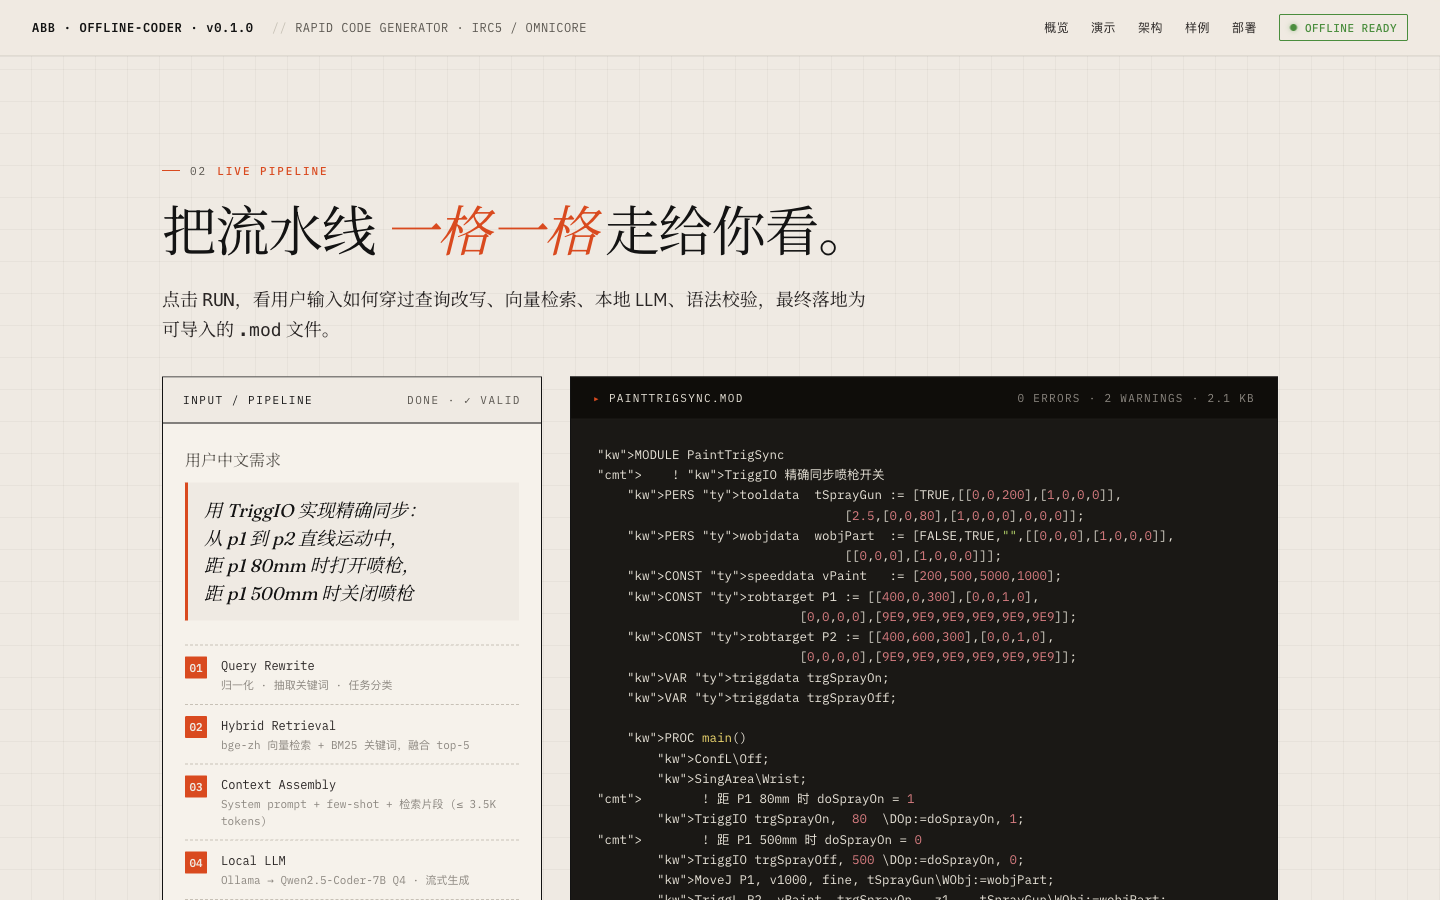
\includegraphics[width=\linewidth]{02-demo.png}\\[2pt]
{\scriptsize 在线演示页：交互式 Pipeline + 真实 .mod 流式输出}
\end{column}
\end{columns}
\takeaway{\textbf{156 测试通过、核心覆盖 92–100\%}，且\textbf{秒级可复现}——工程质量可验证、非 demo。}
\note{\textbf{实测佐证（约 45 秒）—— 讲实在数据}：\textbf{156 测试全过 <1s}，核心覆盖 \textbf{92–100\%}，
\textbf{不需 GPU/Ollama}，任意机器秒级复现。代码 ~4500 行、库 7497 片段、端到端 20–35s。\\
\textit{提示：“可复现”重读；可主动提“佐证材料附了一键复现命令，评委可当场自验”。}}
\end{frame}

% ============ 7. 应用案例 ============
\begin{frame}[fragile]{应用案例：车门 Z 字喷涂（IRC5P）}
\begin{columns}[T]
\begin{column}{0.6\textwidth}
\begin{lstlisting}[style=rapidmini]
MODULE DoorPaint_IRC5P
  PERS tooldata tSprayGun := [...];
  PERS brushdata bdMain := [80,300,50,...];
  PROC main()
    ConfL\Off; SingArea\Wrist;
    ! Z 字扫描 (IRC5P PaintL)
    MoveL p0, v500, fine, tSprayGun\WObj:=wobjPart;
    PaintL p1, vPaint, bdMain, z10, tSprayGun\WObj:=wobjPart;
    ! ... 逐行 Y 偏移 50mm 往返 ...
  ENDPROC
ENDMODULE
\end{lstlisting}
\end{column}
\begin{column}{0.4\textwidth}
\small 一句话\,“600$\times$400 平板 Z 字扫描，行距 50mm”：
\begin{itemize}\small
  \item 自动补全 tooldata/wobjdata/speeddata/brushdata
  \item 安全模板 + 中文注释
  \item 通过静态校验，可直接 Pack\&Go 交付
\end{itemize}
\end{column}
\end{columns}
\takeaway{一句话即\textbf{自动补全全部声明与安全模板}，过校验即可交付——把数小时压到数十秒。}
\note{\textbf{应用案例（约 35 秒）}：一句“600×400 平板 Z 字扫描、行距 50mm” $\to$
\textbf{自动补全} tooldata/wobjdata/speeddata/brushdata + 安全模板 + 中文注释，过校验，可直接 Pack\&Go。\\
\textit{提示：用手指顺一下左侧 \texttt{PaintL}/\texttt{brushdata} 关键行，让评委看到“真能跑”。}}
\end{frame}

% ============ 8. 真实应用现场 ============
\begin{frame}{真实应用现场：本工具生成程序的现场运行}
\begin{columns}[t]
\begin{column}{0.245\textwidth}\centering
  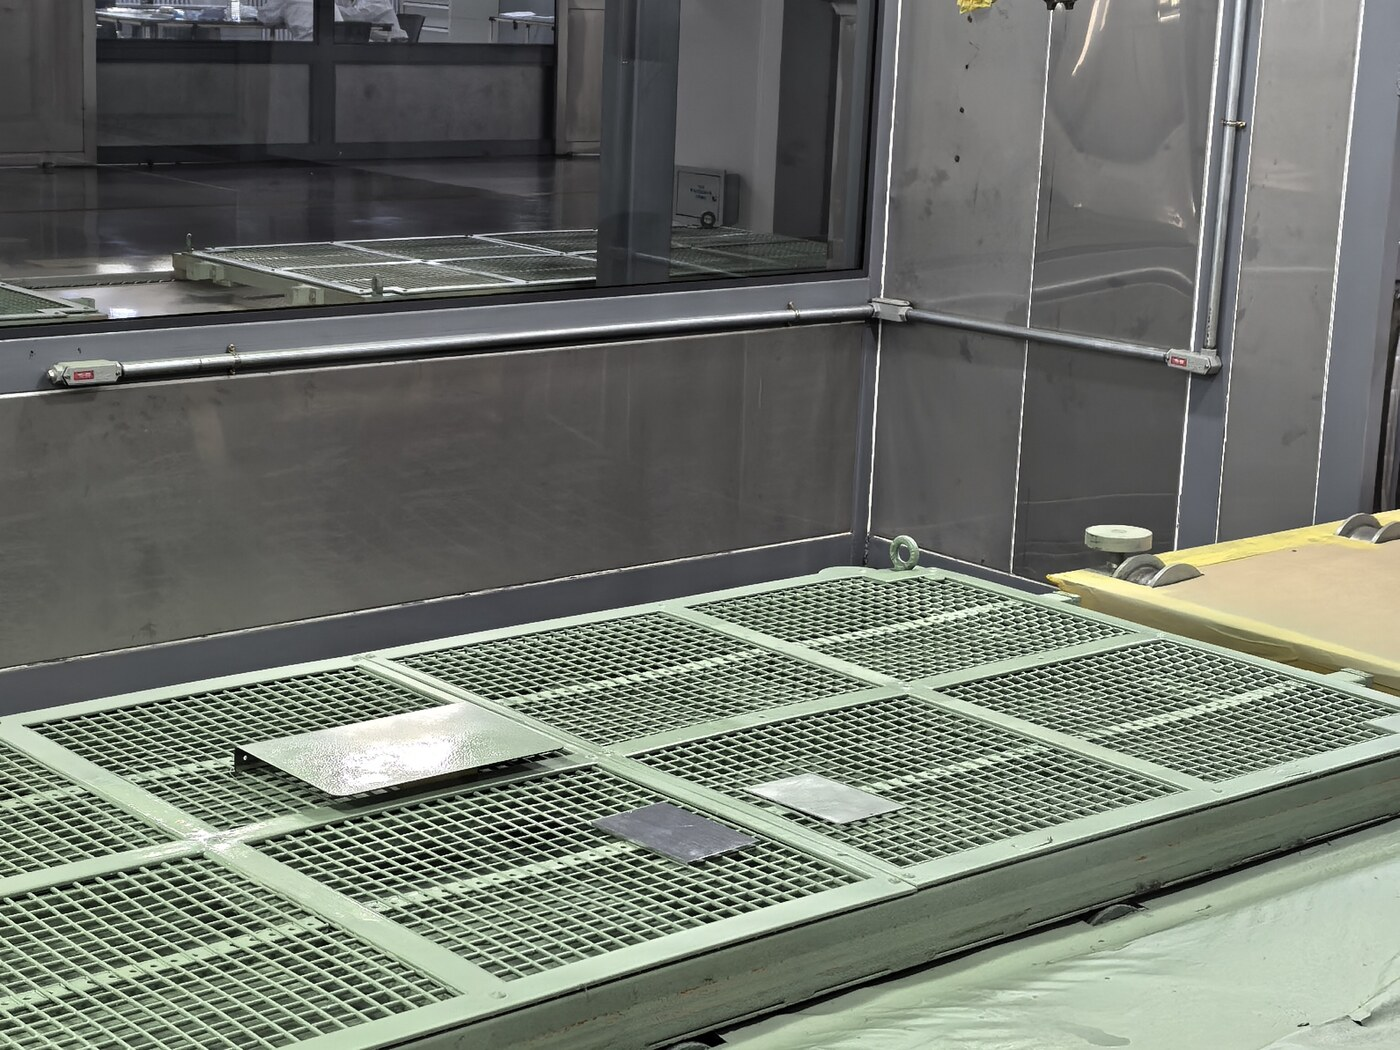
\includegraphics[width=\linewidth]{field-cell.jpg}\\[2pt]{\scriptsize 物理隔离 · 无网玻璃喷房}\end{column}
\begin{column}{0.245\textwidth}\centering
  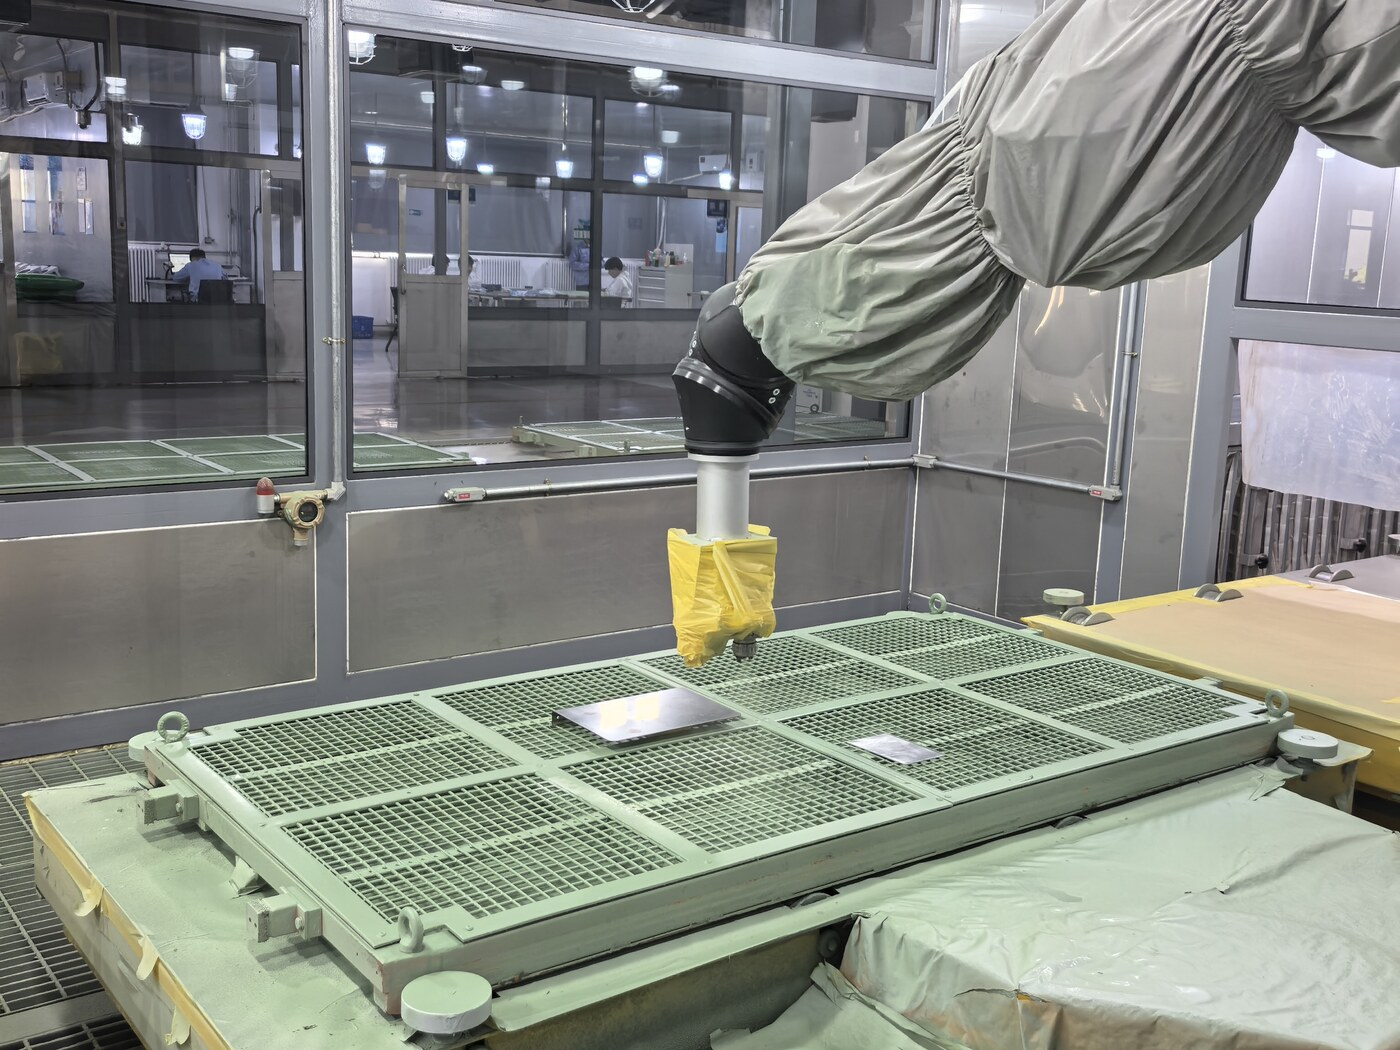
\includegraphics[width=\linewidth]{field-robot.jpg}\\[2pt]{\scriptsize 机器人执行本工具生成程序}\end{column}
\begin{column}{0.245\textwidth}\centering
  
\includegraphics[width=\linewidth]{field-part.jpg}\\[2pt]{\scriptsize 喷涂成品 · 漆面均匀}\end{column}
\begin{column}{0.245\textwidth}\centering
  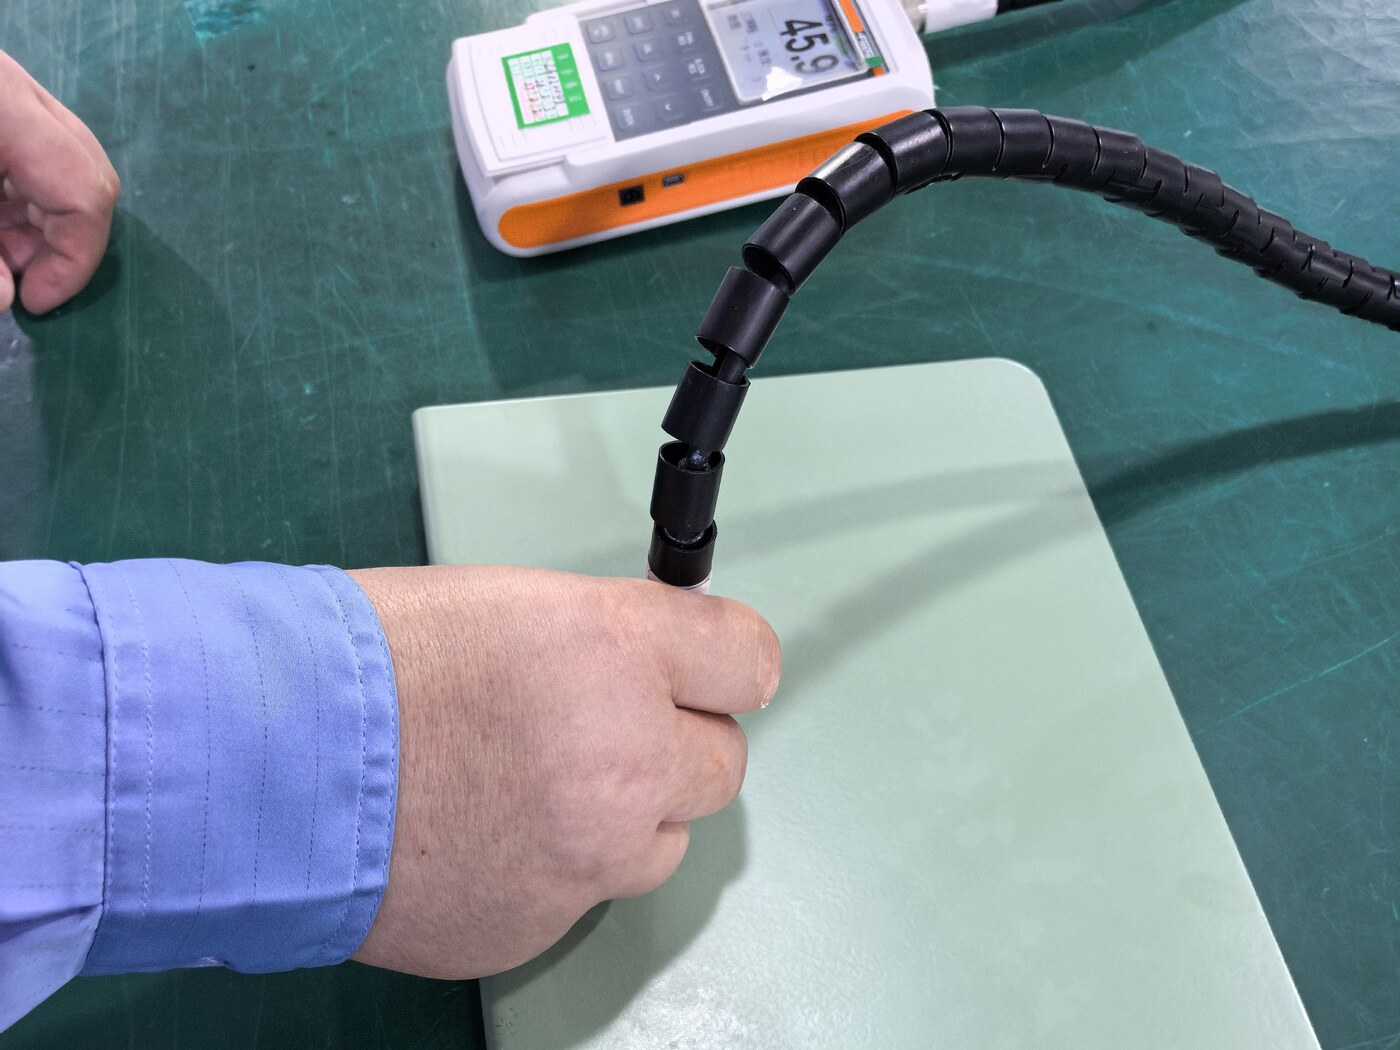
\includegraphics[width=\linewidth]{field-qc.jpg}\\[2pt]{\scriptsize 成品膜厚检测 45.9–61.3\,$\mu$m}\end{column}
\end{columns}
\takeaway{本工具生成的 RAPID 程序\textbf{已在真实（物理隔离、无网）喷涂车间现场运行并通过成品质检}。}
\note{\textbf{真实落地（约 30 秒，强力佐证）}：这不是 demo——左到右是\textbf{真实喷涂车间}：
物理隔离无网玻璃喷房 → 机器人\textbf{执行本工具生成的 RAPID 程序}喷涂工件 → 喷涂成品 → 膜厚检测 \textbf{45.9–61.3\,$\mu$m}。\\
\textit{提示：点出“这是我们工具生成的程序真实跑出来的件”，强调离线落地闭环。}}
\end{frame}

% ====================================================================
\renewcommand{\curphase}{4}
% ============ 9. 创新点 ============
\begin{frame}{创新点总览}
\begin{columns}[T]
\begin{column}{0.5\textwidth}
\begin{enumerate}
  \item 完全离线的工业领域代码生成
  \item 官方手册 RAG 注入，抑制幻觉
  \item IRC5 / IRC5P 双控制器自适应
  \item 生成—校验闭环（11 类规则 + 错误码）
\end{enumerate}
\end{column}
\begin{column}{0.5\textwidth}
\begin{enumerate}
  \setcounter{enumi}{4}
  \item Pack\&Go 一键交付可加载目录
  \item 一键离线迁移（bundle / restore）
  \item 安全护栏内建（TCP/IO/人工复核）
\end{enumerate}
\end{column}
\end{columns}
\takeaway{“\textbf{离线 RAG + 领域校验闭环}”是可复制范式，可迁移至 KUKA KRL、FANUC TP、PLC ST 等封闭工控生态。}
\note{\textbf{创新点（约 30 秒，可加快）}：七点——离线生成、RAG 抑幻觉、双控制器、校验闭环、Pack\&Go、离线迁移、安全护栏。\\
落点在\textbf{“可迁移”}：换知识库/校验规则即可用于 KUKA、发那科、PLC，为总结铺垫。}
\end{frame}

% ============ 10. 总结 ============
\begin{frame}{总结}
\begin{itemize}
  \item 直面喷涂现场\textbf{“无网 + 高门槛”}真实痛点，做\textbf{完全离线}的中文 AI 编程助手
  \item \textbf{本地 LLM + 官方手册 RAG + 生成—校验闭环}，把数小时专家工作压到数十秒
  \item 工程成熟：\textbf{156 测试通过}、核心覆盖 92–100\%、端到端 20–35s、\textbf{现场已落地}
  \item 方法论\textbf{可迁移}到更广的封闭工业机器人 / PLC 生态
\end{itemize}
\vfill
\begin{columns}[c]
\begin{column}{0.66\textwidth}
\begin{center}
{\color{abbgray}\small 源码 \texttt{github.com/Hollis36/abb-offline-coder}\\[2pt]
演示 \texttt{hollis36.github.io/abb-offline-coder}}\\[10pt]
{\Large\bfseries\color{abbred} 谢谢！恳请指正}
\end{center}
\end{column}
\begin{column}{0.3\textwidth}
\begin{center}
\qrcode[height=2.3cm]{https://hollis36.github.io/abb-offline-coder/}\\[4pt]
{\scriptsize\color{abbgray}扫码看在线演示}
\end{center}
\end{column}
\end{columns}
\note{\textbf{总结（约 30 秒）}：无网+高门槛痛点 $\to$ 完全离线中文助手，数小时压到数十秒；
\textbf{156 测试、可复现}；方法论可迁移；已开源。\\
\textit{提示：收尾有力，最后一句放慢、抬头、微笑；停顿后等待提问。随后进入 Q\&A（见讲稿附页）。}}
\end{frame}

\end{document}
